% Malware Workshop
% Copyright (C) 2018  Lilly Chalupowski

% This program is free software: you can redistribute it and/or modify
% it under the terms of the GNU General Public License as published by
% the Free Software Foundation, either version 3 of the License, or
% (at your option) any later version.

% This program is distributed in the hope that it will be useful,
% but WITHOUT ANY WARRANTY; without even the implied warranty of
% MERCHANTABILITY or FITNESS FOR A PARTICULAR PURPOSE.  See the
% GNU General Public License for more details.

% You should have received a copy of the GNU General Public License
% along with this program.  If not, see <https://www.gnu.org/licenses/>.

\documentclass[aspectratio=169]{beamer}
\usepackage{tabularx}
\usepackage{graphicx}
\usepackage{eso-pic}
\usepackage{minted}
\usepackage{hyperref}
\usepackage{tcolorbox}

\makeatletter
\newenvironment{myitemize}{%
  \setlength{\topsep}{0pt}
  \setlength{\partopsep}{0pt}
  \renewcommand*{\@listi}{\leftmargin\leftmargini \parsep\z@ \topsep\z@ \itemsep\z@}
  \let\@listI\@listi
  \itemize
}{\enditemize}
\makeatother

\graphicspath{{img/}}

\usetheme{Warsaw}
\usemintedstyle{monokai}

\setbeamercolor{normal text}{fg=white,bg=black!90}
\setbeamercolor{structure}{fg=white}
\setbeamercolor{alerted text}{fg=red!85!black}
\setbeamercolor{item projected}{use=item,fg=black,bg=item.fg!35}
\setbeamercolor*{palette primary}{use=structure,fg=structure.fg}
\setbeamercolor*{palette secondary}{use=structure,fg=structure.fg!95!black}
\setbeamercolor*{palette tertiary}{use=structure,fg=structure.fg!90!black}
\setbeamercolor*{palette quaternary}{use=structure,fg=structure.fg!95!black,bg=black!80}
\setbeamercolor*{framesubtitle}{fg=white}
\setbeamercolor*{block title}{parent=structure,bg=black!60}
\setbeamercolor*{block body}{fg=black,bg=black!10}
\setbeamercolor*{block title alerted}{parent=alerted text,bg=black!15}
\setbeamercolor*{block title example}{parent=example text,bg=black!15}
\setbeamertemplate{navigation symbols}{}
\setbeamercolor{footercolor}{fg=white,bg=black}

\makeatletter
\defbeamertemplate*{footline}{myfootline}
{
  \leavevmode%
  \hbox{%
    \begin{beamercolorbox}[wd=.333333\paperwidth,ht=2.25ex,dp=1ex,center]{footercolor}%
      \insertshorttitle
    \end{beamercolorbox}%
    \begin{beamercolorbox}[wd=.333333\paperwidth,ht=2.25ex,dp=1ex,center]{footercolor}%
      \insertshortauthor\expandafter\beamer@ifempty\expandafter{\beamer@shortinstitute}{}{~~(\insertshortinstitute)}
    \end{beamercolorbox}%
    \begin{beamercolorbox}[wd=.333333\paperwidth,ht=2.25ex,dp=1ex,right]{footercolor}%
      \insertshortdate{}\hspace*{2em}
      \insertframenumber{} / \inserttotalframenumber\hspace*{2ex} 
    \end{beamercolorbox}}%
  \vskip0pt%
}
\makeatother

\title{Malware Unpacking Workshop}

\institute{GoSecure}
\author{Lilly Chalupowski}
\date{August 28, 2019}

\begin{document}

\setbeamertemplate{footline}{}
\begin{frame}[t]
  \begin{center}
    \begingroup
    \fontsize{20pt}{20pt}\selectfont
    \inserttitle \\
    \endgroup
    \bigskip
    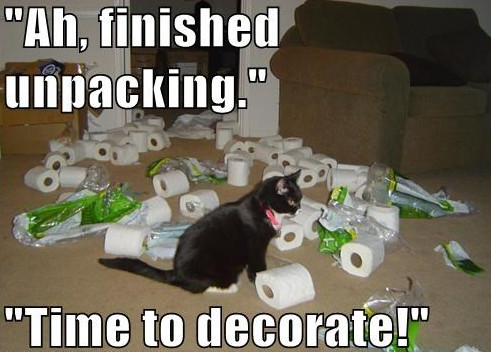
\includegraphics[scale=0.6]{unpacking-cat-meme} \\
    \bigskip
    \insertauthor \\
    \insertdate
  \end{center}
\end{frame}

\setbeamertemplate{footline}[myfootline]

\begin{frame}
  \frametitle{whois lilly.chalupowski}
  \begin{table}
    \caption{\textit{who.is results}}
    \begin{tabularx}{\textwidth}{|X|X|}
      \hline
      Name & Lilly Chalupowski \\
      \hline
      Status & Employed \\
      \hline
      Creation Date & 1986 \\
      \hline
      Expiry & A Long Time from Now (Hopefully)\\
      \hline
      Registrant Name & GoSecure \\
      \hline
      Administrative Contact & Travis Barlow \\
      \hline
      Job & TITAN Malware Research Lead \\
      \hline
    \end{tabularx}
  \end{table}
\end{frame}

\begin{frame}
  \frametitle{Agenda}
  \framesubtitle{What will we cover?}
  \begin{columns}[onlytextwidth]
    \begin{column}{.50\textwidth}
      \begin{itemize}
      \item{Disclaimer}
      \item{Reverse Engineering}
        \begin{itemize}
        \item{Registers}
        \item{Stack}
        \item{Heap}
        \item{Assembly}
        \item{Calling Conventions}
        \end{itemize}
      \item{Tools}
        \begin{itemize}
        \item{x64dbg}
        \item{Cutter}
        \item{Radare2}
        \item{Detect it Easy}
        \item{HxD}
        \end{itemize}
      \end{itemize}
    \end{column}
    \hfill
    \begin{column}{.50\textwidth}
      \begin{itemize}
        \item{Injection Techniques}
          \begin{itemize}
          \item{DLL Injection}
          \item{PE Injection}
          \item{Process Hollowing}
          \item{Atom Bombing}
          \end{itemize}
        \item{Workshop}
      \end{itemize}
    \end{column}
  \end{columns}
\end{frame}

\begin{frame}
  \frametitle{Disclaimer}
  \framesubtitle{Don't be a Criminal}
  \begin{tcolorbox}[title=disclaimer.log,colback=gray]
    The tools and techniques covered in this presentation can be dangerous and are\\
    being shown for educational purposes.\\
    \newline
    It is a violation of Federal laws to attempt gaining unauthorized access to information, assets or systems belonging to others, or to exceed authorization on systems for which you have not been granted.\\
    \newline
    Only use these tools with/on systems you own or have written permission from the owner. I (the speaker) do not assume any responsibility and shall not be held liable for any illegal use of these tools.\\
  \end{tcolorbox}
\end{frame}

\begin{frame}
  \frametitle{Reverse Engineering}
  \framesubtitle{It's easy don't worry!}
  \begin{center}
    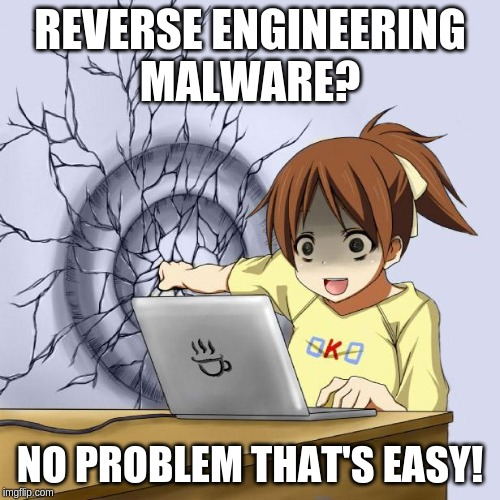
\includegraphics[scale=0.4]{reverse-engineering}
  \end{center}
\end{frame}

\begin{frame}
  \frametitle{Registers}
  \framesubtitle{Not this one!}
  \begin{center}
    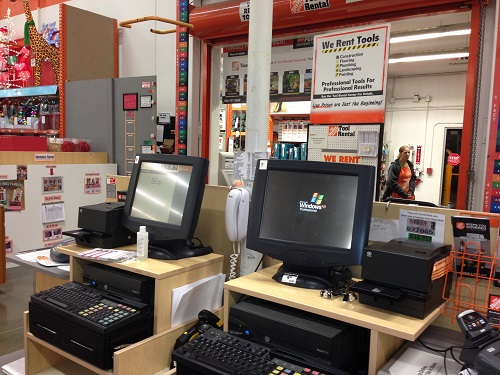
\includegraphics[scale=0.5]{cash-register}
  \end{center}
\end{frame}

\begin{frame}
  \frametitle{Registers}
  \framesubtitle{Not the kind with money in them}
  \begin{columns}
    \begin{column}{.50\textwidth}
      \begin{itemize}
      \item{EAX - Return Value of Functions}
      \item{EBX}
      \item{ECX - Counter in Loops}
      \item{EDI - Destination memory operations}
      \item{ESI - Source memory operations}
      \item{ESP - Stack pointer}
      \item{EBP - Base frame pointer}
      \end{itemize}
    \end{column}
    \hfill
    \begin{column}{.50\textwidth}
      \begin{center}
        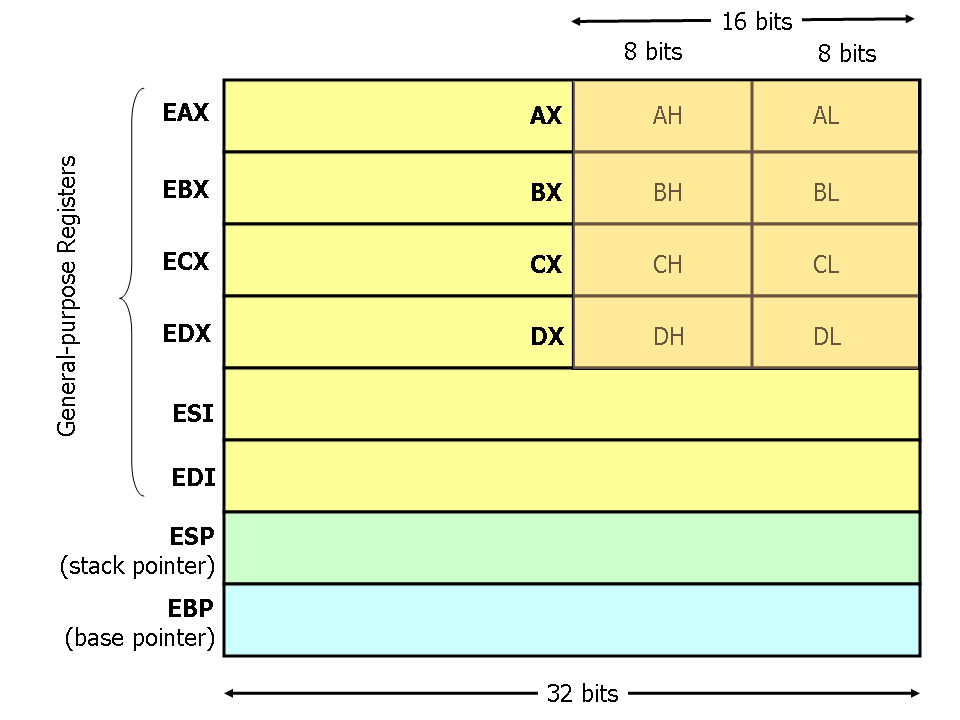
\includegraphics[scale=0.25]{x86-registers}
      \end{center}
    \end{column}
  \end{columns}
  \bigskip
  Did You Know: In computer architecture, a processor register is a quickly accessible location available to a computer's central processing unit (CPU).
\end{frame}

\begin{frame}
  \frametitle{The Stack}
  \begin{columns}
    \begin{column}{.40\textwidth}
      \begin{itemize}
      \item{Last-In First-Out}
        \begin{itemize}
        \item{push}
        \item{pop}
        \end{itemize}
      \item{Downward Growth}
      \item{Function Local Variables}
      \item{ESP}
      \item{Increment / Decrement = 4}
        \begin{itemize}
        \item{Double-Word Aligned}
        \end{itemize}
      \end{itemize}
    \end{column}
    \hfill
    \begin{column}{.60\textwidth}
      \begin{center}
        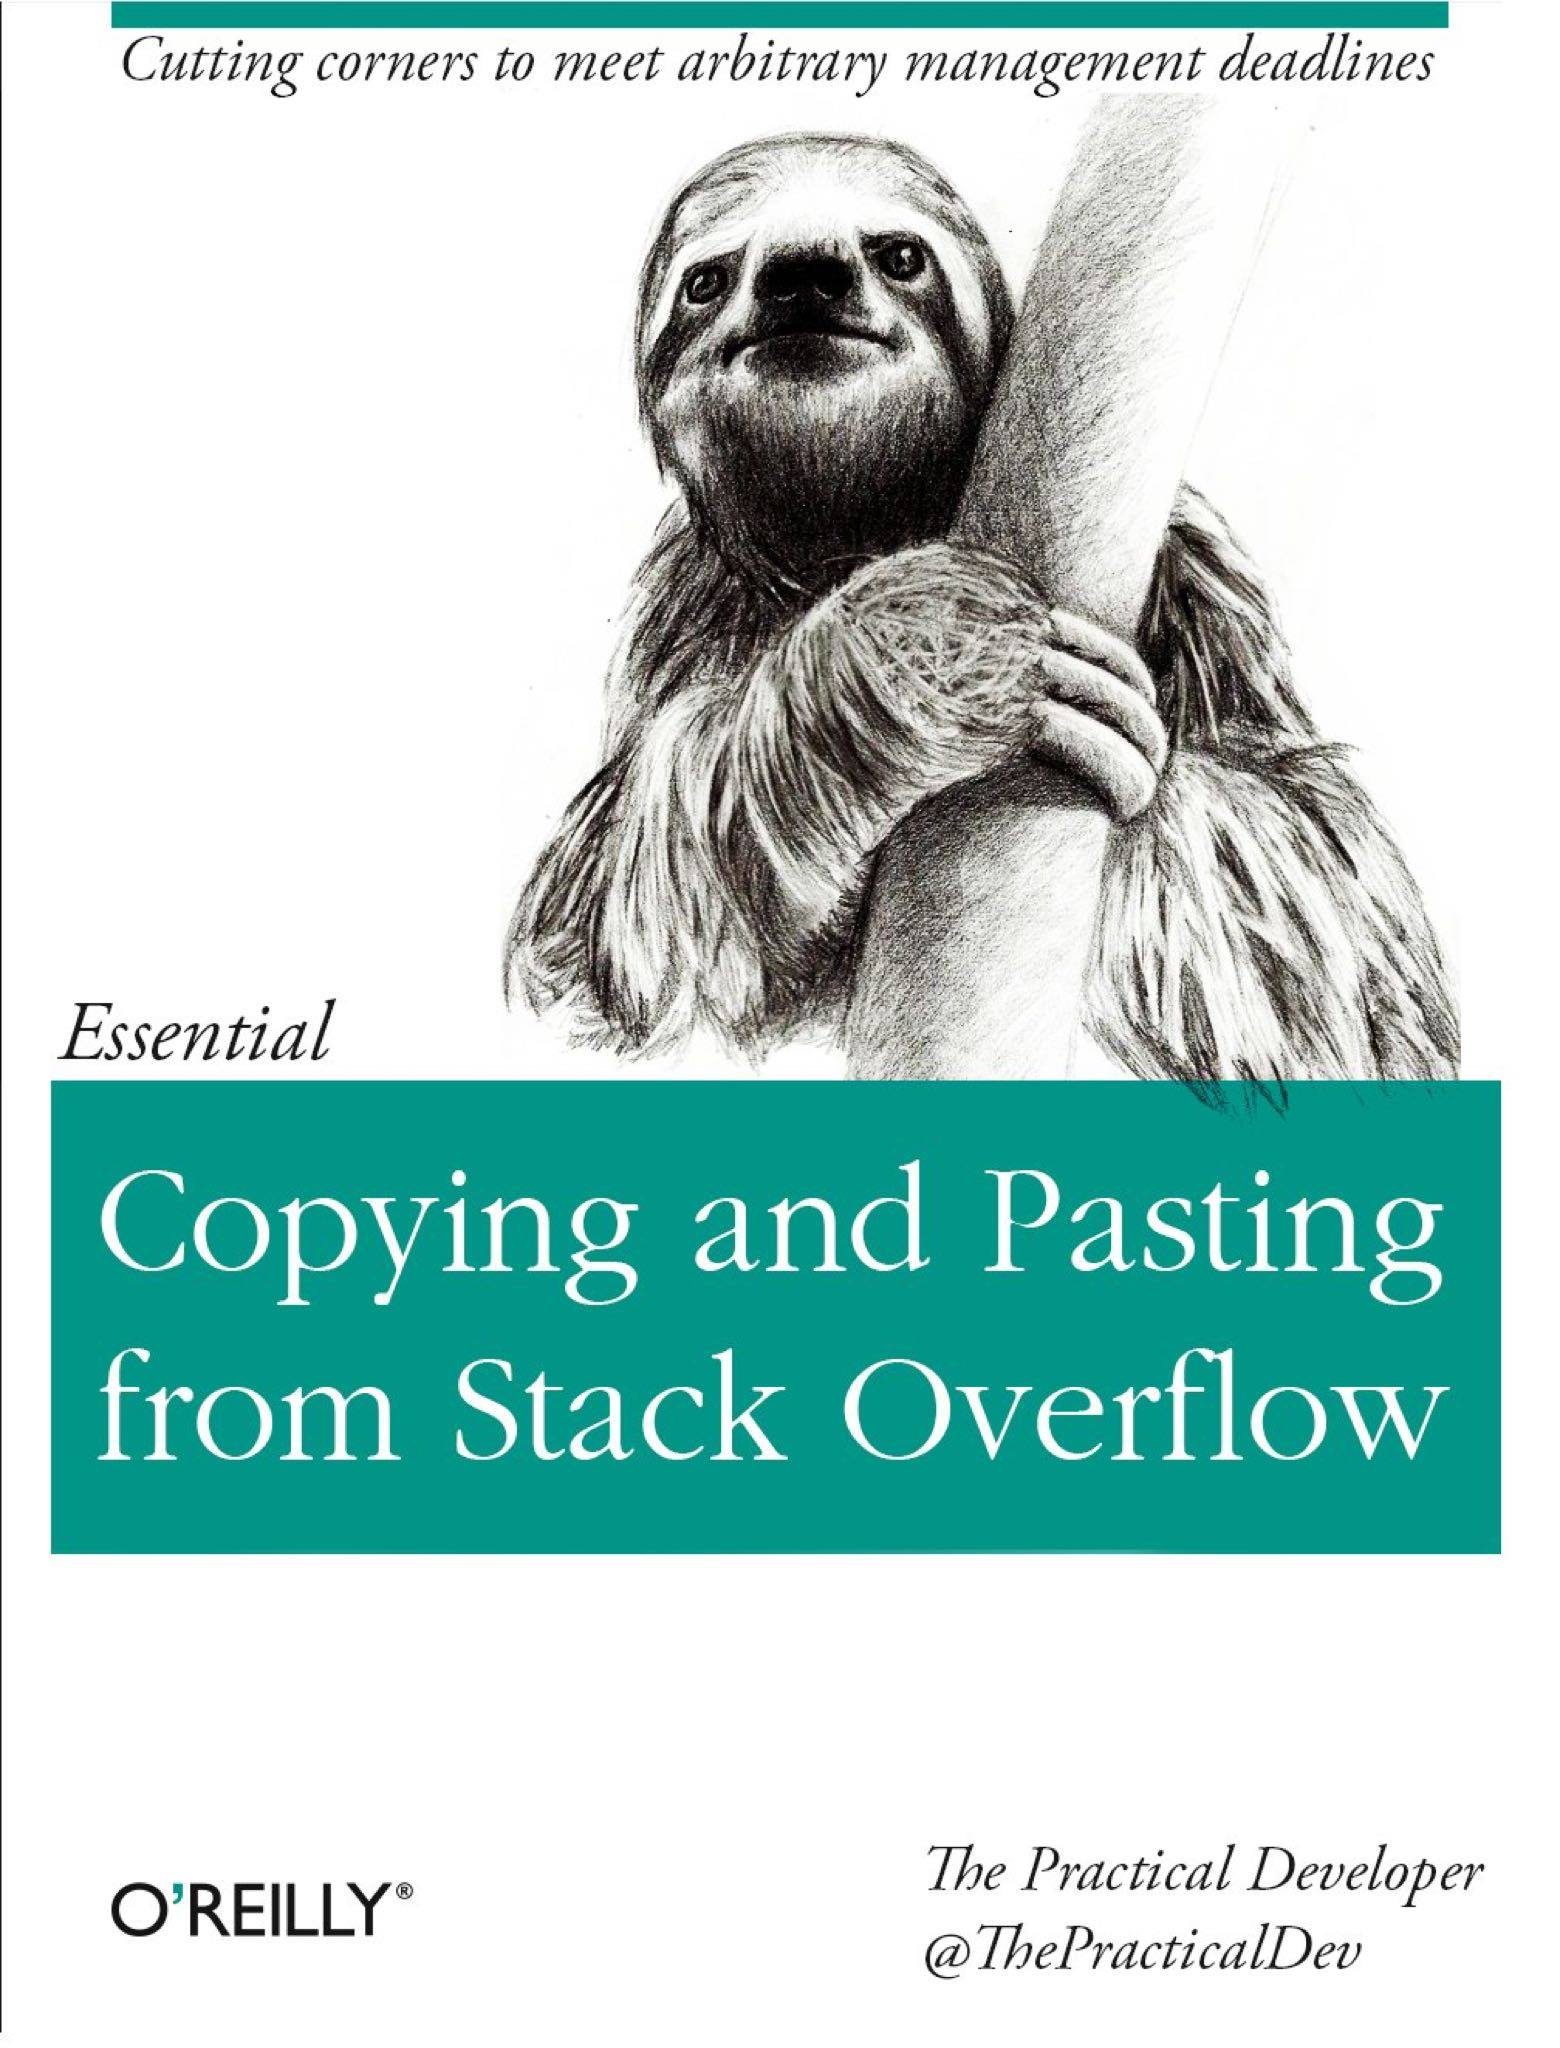
\includegraphics[scale=0.09]{stack-overflow-meme}
      \end{center}
    \end{column}
  \end{columns}
  \end{frame}

\begin{frame}
  \frametitle{Stack}
  \framesubtitle{The stack}
  \begin{center}
    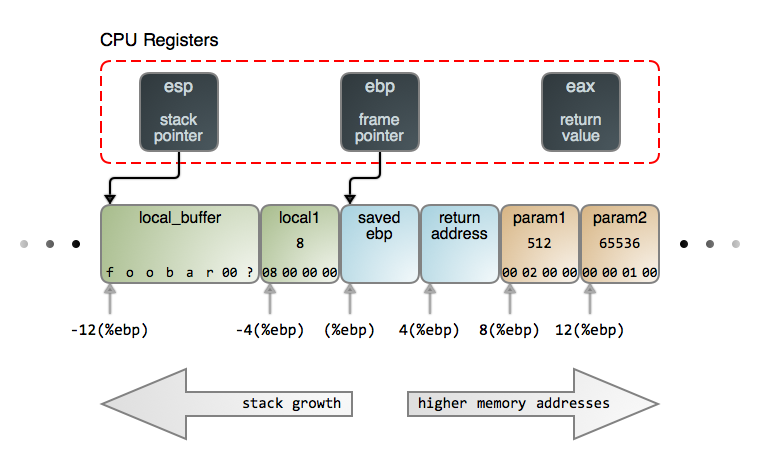
\includegraphics[scale=0.42]{the-stack}
  \end{center}
\end{frame}

\begin{frame}
  \frametitle{Control Flow}
  \framesubtitle{Keeping it under control}
  \begin{columns}
    \begin{column}{.5\textwidth}
      \begin{itemize}
        \item{Conditionals}
          \begin{itemize}
          \item{CMP}
          \item{TEST}
          \item{JMP}
          \item{JCC}
          \end{itemize}
      \item{EFLAGS}
        \begin{itemize}
        \item{ZF / Zero Flag}
          % Set if the result of the previous arithmetic operation is zero
        \item{SF / Sign Flag}
          % Set to the most significant bit of the result
        \item{CF / Cary Flag}
          % Set when the result requires a carry. It applies to unsigned numbers
        \item{OF/Overflow Flag}
          % Set if the result overflows the max size. It applies to signed numbers
        \end{itemize}
      \end{itemize}
    \end{column}
    \hfill
    \begin{column}{.5\textwidth}
      \begin{center}
        
\includegraphics[scale=0.25]{zero-flag-meme}
      \end{center}
    \end{column}
  \end{columns}
\end{frame}

\begin{frame}
  \frametitle{Calling Conventions}
  \framesubtitle{Subtitle goes here}
  \begin{columns}
    \begin{column}{.5\textwidth}
      \begin{itemize}
      \item{CDECL}
        \begin{itemize}
        \item{Arguments Right-to-Left}
        \item{Return Values in EAX}
        \item{Calling Function Cleans the Stack}
        \end{itemize}
      \item{STDCALL}
        \begin{itemize}
        \item{Used in Windows Win32API}
        \item{Arguments Right-to-Left}
        \item{Return Values in EAX}
        \item{The called function cleans the stack, unlike CDECL}
        \item{Does not support variable arguments}
        \end{itemize}
      \item{FASTCALL}
        \begin{itemize}
        \item{Uses registers as arguments}
        \item{Useful for shellcode}
        \end{itemize}
      \end{itemize}
    \end{column}
    \hfill
    \begin{column}{.5\textwidth}
      \begin{center}
        
\includegraphics[scale=0.27]{cdecl-meme}
      \end{center}
    \end{column}
  \end{columns}
\end{frame}

\begin{frame}
  \frametitle{Windows Memory Structure}
  \framesubtitle{subtitle}
  \begin{columns}
    \begin{column}{.6\textwidth}
      \begin{itemize}
      \item{Stack - Grows up to lower addresses}
      \item{Heap - Grows down to higher addresses}
      \item{Program Image}
      \item{TEB - Thread Environment Block}
        \begin{itemize}
        \item{GetLastError()}
        \item{GetVersion()}
        \item{Pointer to the PEB}
        \end{itemize}
        % stores information about the currently running thread
        % The TIB can be used to get a lot of information on the process without calling Win32 API. Examples include emulating GetLastError(), GetVersion(). Through the pointer to the PEB one can obtain access to the import tables (IAT), process startup arguments, image name, etc. It is accessed from the FS segment register when operating on 32 bits, and from GS in 64 bits.
      \item{PEB - Process Environment Block}
        \begin{itemize}
        \item{Image Name}
        \item{Global Context}
        \item{Startup Parameters}
        \item{Image Base Address}
        \item{IAT (Import Address Table)}
        \end{itemize}
        % The PEB contains data structures that apply across a whole process, including global context, startup parameters, data structures for the program image loader, the program image base address, and synchronization objects used to provide mutual exclusion for process-wide data structures. 
      \end{itemize}
    \end{column}
    \hfill
    \begin{column}{.7\textwidth}
      \begin{center}
        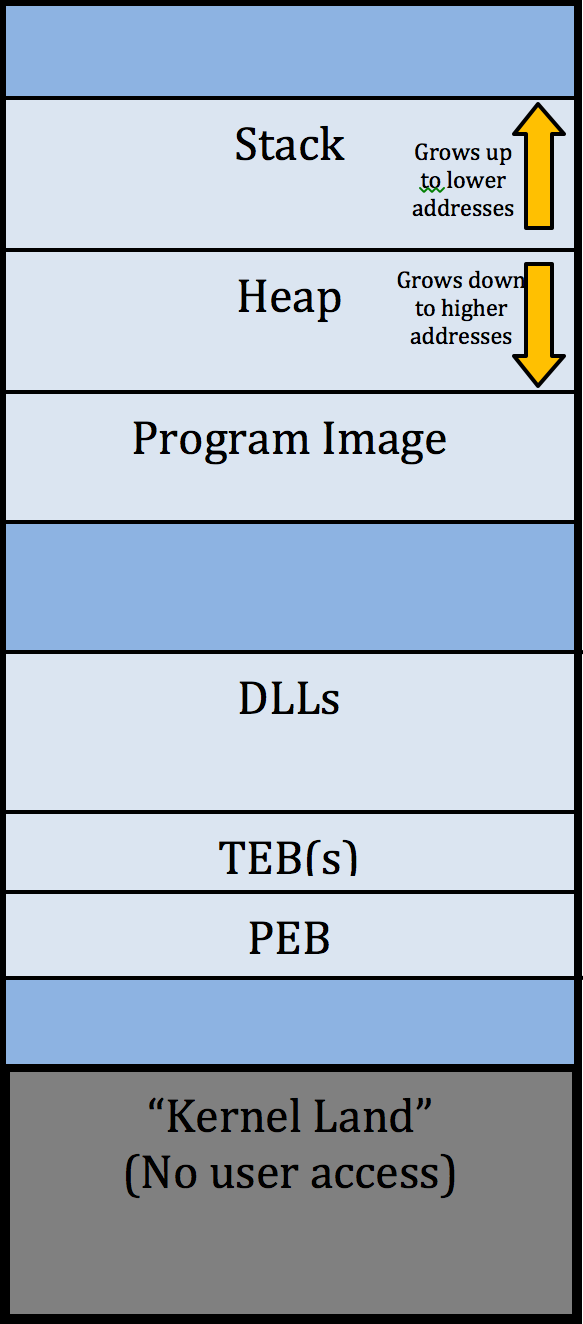
\includegraphics[scale=0.30]{the-heap}
      \end{center}
    \end{column}
  \end{columns}
\end{frame}

\begin{frame}
  \frametitle{Assembly}
  \framesubtitle{Instructions}
  \begin{columns}
    \begin{column}{.3\textwidth}
      \begin{itemize}
      \item{Syntax}
        \begin{itemize}
        \item{Intel}
        \item{AT\&T}
        \end{itemize}
      \item{Common Instructions}
        \begin{itemize}
        \item{MOV}
        \item{XOR}
        \item{IMUL}
        \item{DIV}
        \item{PUSH}
        \item{POP}
      \end{itemize}
      \end{itemize}
    \end{column}
    \hfill
    \begin{column}{0.7\textwidth}
      \begin{center}
        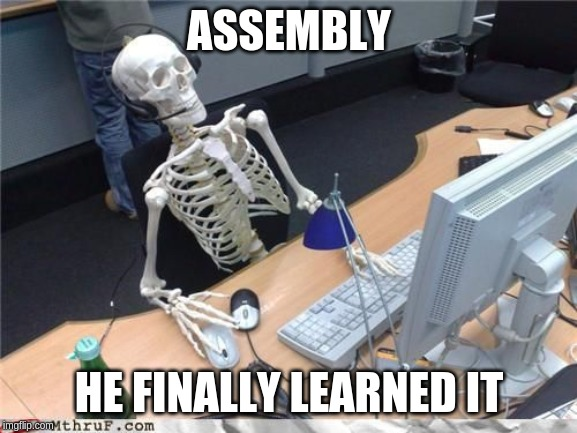
\includegraphics[scale=0.40]{assembly-meme}
      \end{center}
    \end{column}
  \end{columns}
\end{frame}

\begin{frame}
  \frametitle{Assembly Flavors}
  \framesubtitle{I know you were thinking it!}
  \begin{center}
    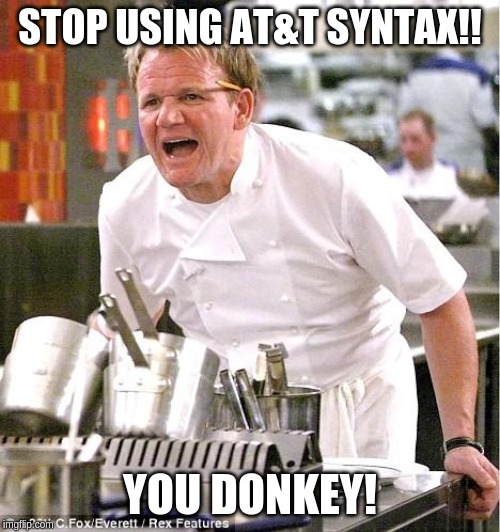
\includegraphics[scale=0.35]{intel-vs-atnt-meme}
  \end{center}
\end{frame}

\end{document}